\documentclass{article}

\PassOptionsToPackage{numbers,sort&compress}{natbib}
\usepackage[main,nonanonymous]{neurips_2026}

\usepackage[utf8]{inputenc}
\usepackage[T1]{fontenc}
\usepackage{hyperref}
\usepackage{url}
\usepackage{booktabs}
\usepackage{amsmath}
\usepackage{amsfonts}
\usepackage{nicefrac}
\usepackage{microtype}
\usepackage{xcolor}
\usepackage{graphicx}
\usepackage{tabularx}
\usepackage{array}

\definecolor{recipientblue}{HTML}{4C78A8}
\definecolor{donororange}{HTML}{E07A3F}
\definecolor{softgray}{HTML}{F2F2F2}
\hypersetup{colorlinks=true,linkcolor=recipientblue,citecolor=recipientblue,urlcolor=recipientblue}

\newcommand{\ours}{reachable-donor future transplantation}
\newcommand{\proj}{\operatorname{proj}}
\newcommand{\kv}{K/V}

\title{How Do World Action Models Use Their Futures? Evidence from Mechanistic Interventions}

\author{Nicole Ma}

\begin{document}

\maketitle

\begin{abstract}
World action models jointly generate future observations and robot actions, but the functional role of their imagined futures remains unclear. Recent destructive interventions establish that these policies causally use future-position representations; they do not show what a particular coherent future tells the policy to do. We introduce reachable-donor future transplantation, which exchanges natural future representations between alternative continuations of the same physical state while fixing the current observation, instruction, action noise, and denoising schedule. The resulting signed estimand asks whether action and physical execution move toward the donor continuation. In Cosmos Policy, donor futures steer actions and executed endpoints at early states across all ten LIBERO-10 tasks; camera and content interventions favor a visible inverse-dynamics account, and effects attenuate sharply at later states. In Cosmos 3, a frozen population study over 22 saved-state clusters and six RoboLab tasks finds predicted-donor action steering of $0.992$ and executed physical steering of $1.003$ on a normalized recipient-to-donor scale. Token-count-preserving activation patching removes $0.877$ of predicted-donor action projection. Yet isolated robot-motion and object-state pixel factors each have effects below $0.011$, despite strong coherent whole-future steering. These results establish cross-generation directional future use and a mediating internal pathway, while showing that the actionable semantic carrier can be distributed or architecture dependent and does not establish general planning over task-object consequences.
\end{abstract}

\section{Introduction}

World action models (WAMs) couple prediction and control: a shared model generates a possible visual future and the robot action to take next \citep{guo2024pad,hu2025vpp,li2025uva,kim2026cosmospolicy,ye2026dreamzero}. This architecture invites a planning-like interpretation. The policy appears to imagine how the scene could evolve and then act using the anticipated consequences. Joint generation alone, however, does not identify this computation. The future could be behaviorally irrelevant, could act as an undifferentiated latent workspace, or could mainly encode the robot motion already paired with the action.

RIFT substantially narrows this ambiguity \citep{zhang2026rift}. Across four WAMs and all 40 LIBERO tasks, masking or reassigning future-cache values changes executed trajectories and reduces success. RIFT therefore establishes that WAM action experts causally use meaningful, position-bound future representations. It does not show what a particular coherent future tells the policy to do. Its principal intervention outcomes are deviation from the original execution and task success: they reveal dependence, but do not associate an edited future with a specific alternative behavior and ask whether the robot moves toward it.

We make that question directional. From one exactly restored physical state, two native policy branches define a recipient and donor: alternative generated futures, actions, and executed endpoints that are all reachable from the same state. We insert the donor future into the recipient computation and score the result on the signed recipient-to-donor axis. If the future merely perturbs computation, behavior may change without aligning to the donor. If its content controls action, the patched action and endpoint should move toward the particular behavior associated with the donor. Multiple donors further test whether the intervention selects the correct alternative.

This distinction can be stated compactly: \emph{RIFT establishes future dependence; we test semantic directionality.} Figure~\ref{fig:overview} summarizes the design. We combine representation transplantation with modality and object/robot content interventions, destructive attention localization, and token-count-preserving activation patching of future-token keys and values. This yields three linked questions: (i) can coherent future content directionally select behavior, (ii) what content carries that effect, and (iii) through which internal interface does it act?

\begin{figure}[t]
  \centering
  
\includegraphics[width=\linewidth]{figures/method_overview.pdf}
  \caption{Reachable-donor future transplantation gives a destructive intervention a semantic direction. (a) Two policy-native continuations start at the exact same state. (b) The recipient run retains its current observation, instruction, noise, and schedule, but receives the donor future. (c) signed projections test movement toward that donor; activation patching then tests whether future-token \kv{} content mediates the effect.}
  \label{fig:overview}
\end{figure}

We find strong but bounded future use. At the first decision state in Cosmos Policy, donor futures steer action and physical execution in all ten LIBERO-10 tasks. Wrist imagery carries most of the effect, primary-camera imagery carries a smaller effect, and future proprioception is null. The effect falls sharply at later registered states. A separate 20-state $2\times2$ intervention changes decoded robot and object futures with high target specificity but produces essentially no object-content effect. Rare natural robot-only pairs steer strongly; matched object-only pairs do not reliably identify their donor. In the released Cosmos 3 policy, predicted and physically executed donor futures steer action and robot execution across 22 independent clusters and all six eligible RoboLab tasks. Replacing donor-run future-token \kv{} with self-future \kv{} suppresses donor steering and physical execution in every cluster. A separate masked $2\times2$ study, however, finds that neither isolated robot pixels nor isolated object pixels reproduce a meaningful fraction of the whole-future effect.

The result is mechanistic at the representation and pathway level, not a complete circuit account. Both policies use coherent imagined visual futures to steer action, but the content carrier differs: Cosmos Policy evidence favors prospective visible robot motion, whereas Cosmos 3 requires a more compositional or distributed account. We do not find evidence that either model generally evaluates task-object consequences, searches over plans, or selects successful futures.

\section{Related work}

\paragraph{World action models.}
Joint image/action denoising and predictive visual policies learn futures alongside controls \citep{guo2024pad,hu2025vpp,li2025uva}. Cosmos Policy fine-tunes a pretrained video model for future prediction and visuomotor control \citep{kim2026cosmospolicy}; Cosmos 3 provides a later omnimodal architecture and released DROID policy \citep{nvidia2026cosmos3}. These architectures establish that future and action can be generated together, not what downstream computation uses the future for.

Recent efficiency work exposes the same ambiguity. Fast-WAM shows that explicit test-time rollout can be removed while retaining competitive performance \citep{yuan2026fastwam}; Faster-WAM retains efficient future conditioning for robustness \citep{zhao2026fasterwam}. AGRA argues that visually plausible foresight need not be action-grounded and modifies training to improve representation alignment \citep{qiu2026agra}. These results distinguish the benefits of future-prediction training from the use of a particular generated future at inference.

\paragraph{Closest comparison: RIFT.}
RIFT records and edits the action-independent future-position \kv{} interface \citep{zhang2026rift}. Masking, norm-matched noise, frozen-present values, and spatial or temporal reassignment cause large trajectory drift and success loss. Replaying one final-clean cache nearly preserves execution in supported architectures, establishing consumption-side sufficiency of a fixed interface. Our question begins after that result. RIFT asks whether meaningful future values and their positions are required; we ask whether a coherent alternative future selects its associated alternative action and physical endpoint. Its EE-ADE is an unsigned deviation from the original trajectory. Our donor projection is signed by an independently generated alternative.

\paragraph{Mechanistic interventions.}
Causal mediation distinguishes information that is encoded from information actually used downstream \citep{pearl2001direct,vig2020causalmediation}. Causal tracing and path patching localize behavior by replacing internal activations or computational routes \citep{meng2022rome,goldowskydill2023pathpatching}. Activation-patching methodology motivates clean/corrupted pairing, explicit metrics, no-op controls, and held-out validation \citep{zhang2024activationpatching}. Because patched components can interact with unpatched mediators, we interpret layer and group effects as bounded pathway evidence rather than additive circuit decomposition \citep{vaidyanathan2026multiplemediators}.

\section{Experimental logic}

\subsection{Reachable-donor transplantation}

Let state $S$ admit two native branches $A$ and $B$. Their generated action chunks are $a_A,a_B$, their future representations are $F_A,F_B$, and physical execution yields endpoints $e_A,e_B$. We rerun recipient $A$ while holding fixed $S$, the language instruction, recipient action noise, future-noise path, solver, and denoising schedule. Only the clean future target changes from $F_A$ to $F_B$.

For an intervened action $\hat a$, normalized donor projection is
\begin{equation}
  \pi_a(\hat a;A,B)=
  \frac{(\hat a-a_A)^\top(a_B-a_A)}{\lVert a_B-a_A\rVert_2^2}.
  \label{eq:projection}
\end{equation}
Thus native recipient $A$ is 0 and native donor $B$ is 1; negative values move away from $B$, and values above 1 overshoot it. We define $\pi_e$ analogously for registered physical endpoints. The principal contrast is donor clamp minus self clamp, averaged over reciprocal branch directions and future-noise draws within saved state. This signed estimand is the central difference from generic disruption.

Pairs are selected using only native action and endpoint separation, never intervention outcomes. Controls include an exact self clamp, an exact norm- and recipient-distance-matched Gaussian target, a prespecified natural control, a within-task shuffled future, and bitwise no-op recomputations. We separately clamp wrist video, primary video, and future proprioception. Every saved action condition is executed from the exact simulator state.

\subsection{What content is used?}

The initial transplant contains several correlated signals: robot pose, object state, camera motion, and potentially task progress. We therefore use two complementary designs. A natural-pair screen searches for robot-divergent/object-matched and object-divergent/robot-matched futures from a common recipient. These are policy-native but structurally rare. A separately frozen $2\times2$ study re-renders object state $O\in\{0,1\}$ crossed with robot state $R\in\{0,1\}$ at 20 held-out LIBERO states. This achieves broad coverage and exact factor preservation, but its hybrid videos may be off the native future manifold. We report both rather than treating one as definitive.

\subsection{Pathway interventions}

In Predict2-based Cosmos Policy, action queries can attend to future keys. We remove future keys at a prespecified late transformer block with a continuous gate, alongside all-key identity, random-key, current-key, and early-block controls. This is a necessity/localization test and changes attention normalization.

Cosmos 3 permits a cleaner content-mediation test. We first record future-video keys and values from a self-future run. During a donor-future run, we replace only future-token \kv{} at selected layers; token count, token order, current-video \kv{}, text \kv{}, action \kv{}, current observation, instruction, and noise remain unchanged. Record/replay and self-patch arms must be bitwise exact. If donor projection falls after the patch, the replaced future content mediates that donor-directed effect. We report the absolute reduction in donor projection (``mediation loss''), not a population natural indirect effect.

\begin{table}[t]
  \caption{Each intervention answers a different causal question. The donor experiment adds a signed semantic target that destructive tests do not provide.}
  \label{tab:logic}
  \centering
  \small
  \begin{tabularx}{\linewidth}{@{}>{\raggedright\arraybackslash}p{0.21\linewidth}>{\raggedright\arraybackslash}p{0.30\linewidth}>{\raggedright\arraybackslash}X@{}}
    \toprule
    Intervention & Primary readout & Supported conclusion \\
    \midrule
    Mask/noise/shuffle & trajectory drift; success & future-interface dependence \\
    Reachable donor & signed action and endpoint projection & content-specific directional sufficiency \\
    Modality/$2\times2$ content & donor projection under isolated content & functional content used by the policy \\
    Self-\kv{} patch into donor run & loss of donor-directed projection & pathway-level content mediation \\
    \bottomrule
  \end{tabularx}
\end{table}

\subsection{Statistical inference}

The independent unit is an exactly restored simulator state. Reciprocal directions, multiple donors, noise draws, and process repeats are repeated measurements. Unless stated otherwise, intervals are 10,000-resample cluster bootstraps over saved states; task-balanced sensitivities first average states within task and then bootstrap tasks. We preregistered 0.10 donor-projection units---ten percent of the native recipient-to-donor displacement---as the smallest effect of interest for the Predict2 confirmatory family and the Cosmos 3 population and factor families. Registered primary-family sign tests receive Holm correction.

\section{Do alternative futures directionally steer actions?}

\subsection{Cosmos Policy: population-level test}

We first study the released \texttt{Cosmos-Policy-LIBERO-Predict2-2B} checkpoint \citep{kim2026cosmospolicy} on LIBERO-10 \citep{liu2023libero}. The frozen grid contains 30 unseen units: ten tasks crossed with a first query, a state after three open-loop chunks, and a state after six chunks. Eight native branches determine one reciprocal donor pair per state. Three future-noise draws are repeated within direction. Physical endpoints concatenate goal-relevant simulator coordinates with the official nine-dimensional proprioceptive endpoint. Pair selection, controls, attention block, outcome construction, and bootstrap are frozen before intervention outcomes.

At the first query, donor-minus-self action steering is $0.499$ (95\% CI $[0.336,0.679]$), positive in all ten tasks. Executed endpoint steering is $0.552$ ($[0.387,0.728]$), also positive in all ten. The action contrast remains positive against Gaussian ($0.497$), prespecified natural ($0.103$), and shuffled-future ($0.255$) controls. Physical contrasts are respectively $0.549$, $0.110$, and $0.277$. This is not merely an action-vector change: the simulator endpoint moves in the independently defined donor direction.

The effect is state dependent (Figure~\ref{fig:predict2}a). After three chunks, mean action steering falls to $0.031$ and physical steering to $0.004$. After six chunks they are $0.027$ and $0.025$. Across all 30 registered states, action steering is $0.186$ ($[0.095,0.290]$) and physical steering is $0.194$ ($[0.091,0.305]$), but the lower intervals narrowly miss the 0.10 practical threshold. Because each timing stratum uses a different initial-state index, this is a state/timing association rather than a pure causal effect of elapsed time. The supported claim is strong steering at identifiable early states, not uniform future mediation throughout an episode.

\begin{figure}[t]
  \centering
  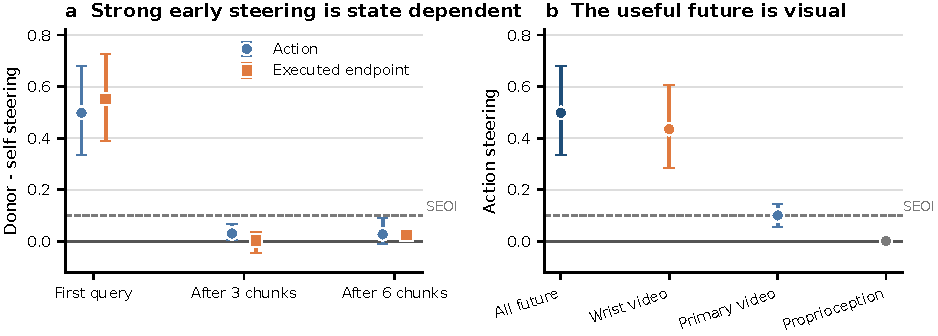
\includegraphics[width=\linewidth]{figures/predict2_results.pdf}
  \caption{Predict2-based Cosmos Policy uses visual futures strongly at early states. Points are saved-state means and bars are 95\% cluster-bootstrap intervals. (a) action and executed endpoint steering are large at the first query and sharply attenuate at later registered states. (b) wrist video carries most first-query action steering, primary video carries a smaller effect, and future proprioception is null. SEOI: preregistered smallest effect of interest (0.10).}
  \label{fig:predict2}
\end{figure}

\subsection{Cosmos 3: cross-generation replication}

We port the same reachable-donor logic to the released 16B \texttt{Cosmos3-Nano-Policy-DROID} checkpoint \citep{nvidia2026cosmos3} and public RoboLab tasks \citep{yang2026robolab}. Cosmos 3 uses 36 two-way full-attention layers, four UniPC denoising calls, 33 raw video frames mapped to nine VAE latent frames, and 32 absolute joint-position actions. The intervention targets only unconditioned future-video coordinates at the final guided sampler boundary. Identity layout capture, identity sampler wrapping, cache record/replay, and self patches reproduce actions bitwise; sentinels verify zero direct mutation of action coordinates. Each physical condition reconstructs the environment, restores the same initial state, and replays the prefix exactly.

Before inspecting confirmatory interventions, a frozen native census selected 24 saved-state clusters across six eligible tasks, capped at four per task, using only native success, action and endpoint separation, and replay validity. Twenty-two clusters completed. Two registered native branches terminated before producing the full 33-frame videos required as intervention sources; these units remain missing and were not replaced. The prespecified minimum of 20 clusters across five tasks was therefore achieved. The independent unit is saved state; reciprocal directions and source types are repeated measures.

Predicted-donor action steering is $0.992$ (95\% state-bootstrap CI $[0.972,1.010]$), positive in 22/22 clusters and every task. It remains $0.433$ ($[0.332,0.538]$) above a preselected natural-future control. For futures encoded from physically executed reachable branches, donor-minus-executed-self action steering is $0.983$ ($[0.890,1.064]$), and executed physical endpoint steering is $1.003$ ($[0.950,1.050]$), both positive in 22/22 clusters. Executed-donor action steering also exceeds the geometry-matched Gaussian by $0.941$ ($[0.837,1.032]$) and the natural control by $0.391$ ($[0.246,0.533]$). Task-balanced bootstraps agree with every conclusion. All registered primary donor and \kv{} sign tests remain positive after Holm correction.

The four-task multi-donor engineering study additionally verifies correct-alternative specificity: action identifies the correct donor in 12/12 cases for predicted and executed sources. The population result now establishes cross-task generality in a later, substantially different policy rather than only repeated engineering feasibility. It still does not identify mediation of task success: no screened branch pair in either policy retained a robust binary success/failure label across continuation seeds.

\begin{table}[t]
  \caption{Main signed effects organized by scientific question. Intervals cluster on saved state.}
  \label{tab:results}
  \centering
  \small
  \begin{tabularx}{\linewidth}{@{}>{\raggedright\arraybackslash}p{0.22\linewidth}>{\raggedright\arraybackslash}p{0.14\linewidth}>{\raggedright\arraybackslash}p{0.27\linewidth}>{\raggedright\arraybackslash}X@{}}
    \toprule
    Study & Units & Effect (95\% CI) & Main reading \\
    \midrule
    Predict2 first query & 10 states & action: $0.499$ $[0.336,0.679]$ & coherent donor selects action \\
    Predict2 first query & 10 states & endpoint: $0.552$ $[0.387,0.728]$ & direction survives execution \\
    Cosmos 3 population & 22 states, 6 tasks & action: $0.992$ $[0.972,1.010]$ & all predicted donors steer \\
    Cosmos 3 population & 22 states, 6 tasks & physical: $1.003$ $[0.950,1.050]$ & direction survives execution \\
    Predict2 visual content & 10 states & wrist: $0.435$ $[0.284,0.605]$ & visual robot motion dominates \\
    Predict2 $2\times2$ object & 20 states & action: $0.00015$ $[-0.00012,0.00049]$ & isolated object content is null \\
    Natural robot-only & 4 states & action: $0.291$ $[0.060,0.521]$ & strong but exploratory \\
    Cosmos 3 predicted-future \kv{} patch & 22 states, 6 tasks & loss: $0.877$ $[0.842,0.910]$ & future \kv{} mediates direction \\
    Cosmos 3 pixel factors & 10 states, 6 tasks & robot: $0.0022$; object: $0.0061$ & neither isolated factor is meaningful \\
    \bottomrule
  \end{tabularx}
\end{table}

\section{What information in the future causes the steering?}

\subsection{Visual modalities}

Modality clamps localize the early result to vision (Figure~\ref{fig:predict2}b). Wrist-future action steering is $0.435$ ($[0.284,0.605]$), primary-camera steering is $0.101$ ($[0.057,0.144]$), and future-proprioception steering is $0.001$ ($[-0.004,0.008]$). Because the wrist view tightly tracks the manipulator, this pattern predicts a prospective visible-motion or inverse-dynamics-like role.

\subsection{Robot-motion versus object-state content}

The content studies support that interpretation while exposing its limits. In the 20-state $2\times2$ study, decoded futures identify the intended target cell with 92.5\% primary-camera and 98.75\% wrist-camera top-1 accuracy. Nevertheless, the object main effect is $0.00015$ on action similarity ($[-0.00012,0.00049]$) and $0.00018$ on executed goal-state steering ($[-0.00040,0.00102]$), far below 0.10. Endpoint target-cell identification is exactly chance (0.25). The manipulation changes the decoded object future, but execution does not follow it.

Natural matching avoids rendered hybrids but yields only four eligible units, below the frozen minimum of ten. In those units, robot-only future transplantation gives action steering $0.291$ ($[0.060,0.521]$) and executed robot-endpoint steering $0.315$ ($[0.059,0.571]$). Object-only effects are much weaker: action $0.021$ and goal endpoint $0.021$ with an interval crossing zero; correct-donor top-1 is at each unit's chance rate. We therefore do not infer that object consequences are universally unused. We infer that the observed steering is best explained by prospective visible robot motion, while meaningful isolated object-state use is unsupported in these experiments.

This content conclusion is deliberately narrower than the directional result. Natural object-only alternatives are rare, whereas rendered $2\times2$ hybrids may lie off the policy's native future manifold. Donor videos also contain robot pose and correlated visual changes. ``Prospective visible robot motion'' is therefore the best-supported functional description at the studied Cosmos Policy states, not a fully decoded latent variable or a universal claim that WAMs ignore object consequences.

Cosmos 3 provides an important counterpoint. A separately frozen factor family selects 12 population units round-robin by native object-position separation; ten complete across all six tasks, meeting its prespecified minimum. Starting from the native recipient video, an object-priority disjoint mask copies donor object pixels, donor robot pixels outside the object mask, both, or neither. The isolated robot main effect is $0.0022$ on action ($[-0.0016,0.0060]$) and $0.0102$ on the full executed endpoint ($[-0.0067,0.0275]$). The isolated object effect is $0.0061$ on action ($[0.0009,0.0119]$) and $-0.0001$ on the full endpoint ($[-0.0254,0.0239]$). Every interval lies inside the preregistered $\pm0.10$ equivalence region, and task-balanced estimates agree. The detectable object action effect is only 0.6\% of native donor displacement and is practically negligible. Small-denominator object-specific endpoint ratios are unstable and are not used for equivalence claims.

Thus strong whole-future steering does not reduce to either isolated pixel factor in Cosmos 3. This cross-model difference rules out a universal robot-pixel account: actionable content may require coherent robot--object context, be distributed outside the masks, or interact nonlinearly with tokenization. The study does not show that robot and object factors are jointly necessary.

\section{Through what internal pathway does the future affect action?}

\subsection{Cosmos Policy: an active future-to-action attention edge}

Removing future keys from action queries at block 27 yields a monotonic action-disruption curve: normalized L2 is 0.022, 0.035, 0.054, and 0.068 at gates 0.25, 0.50, 0.75, and 1.00. The all-key recomputation is bitwise exact. Full removal is more disruptive than equal-count random-key removal by $0.016$ and than block-0 future removal by $0.048$. Equal-count current-key removal is larger by $0.024$. Executed endpoints show the same bounded conclusion: the late future edge is causally active, but neither the only nor the largest route through the block.

\subsection{Cosmos 3: future-token K/V content mediates steering}

Layer and pathway choice are frozen from excluded calibration tasks, where direct-interface patching removes $0.842$ projection units ($[0.766,0.910]$) and exact record/replay and self-patch gates pass. In the confirmatory population, predicted-future \kv{} replacement removes $0.877$ action-projection units ($[0.842,0.910]$), positive in 22/22 clusters. Executed-future replacement removes $0.814$ action units ($[0.723,0.900]$) and $0.851$ physical-endpoint units ($[0.766,0.922]$), again positive in every cluster. Task-balanced estimates are $0.877$, $0.812$, and $0.853$, with intervals excluding zero and the 0.10 smallest effect of interest. All primary family sign tests survive Holm correction.

Together, the two models provide complementary pathway evidence rather than identical circuit analyses. Cosmos Policy shows that a late future-to-action attention edge is necessary enough to measurably affect behavior. Cosmos 3 preserves token count and attention normalization while replacing future-token content, giving stronger evidence that donor-directed information is mediated through future-token \kv{}. Layerwise and grouped patches can still interact with unpatched mediators \citep{vaidyanathan2026multiplemediators}; they identify an active internal pathway, not a complete or uniquely necessary circuit.

\begin{figure}[t]
  \centering
  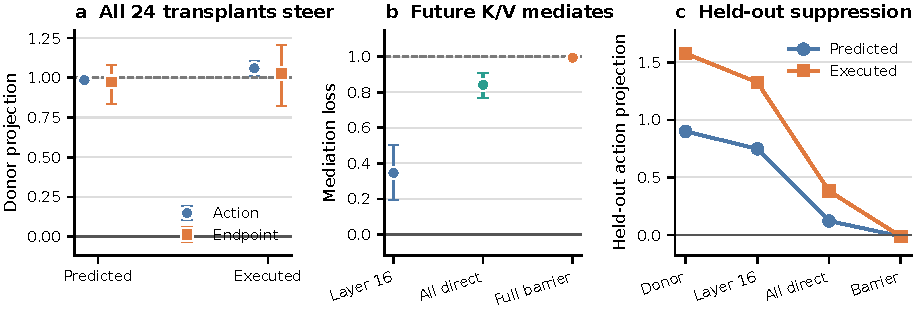
\includegraphics[width=\linewidth]{figures/cosmos3_results.pdf}
  \caption{Cosmos 3 population results. Points and bars are saved-state means and 95\% cluster-bootstrap intervals. (a) coherent predicted and executed futures steer action, beat natural controls, and move physical endpoints toward the donor across 22 clusters and six tasks. (b) token-count-preserving self-future \kv{} replacement removes most donor steering. (c) in ten factor units across six tasks, isolated robot and object pixels have effects within the preregistered $\pm0.10$ equivalence region.}
  \label{fig:cosmos3}
\end{figure}

\section{Discussion}

\paragraph{What is the imagined future for?}
The shared account across models is prospective visual action conditioning: a particular coherent future specifies a corresponding action direction, and the policy reads this relation through future-token content. Cosmos Policy further resembles visually mediated inverse dynamics: the strongest modality is the wrist camera, natural robot-only donors steer strongly, and future proprioception and isolated object-state content do not \citep{hu2025vpp}. Cosmos 3 does not admit the same isolated-pixel explanation. Its whole future steers almost completely while robot-only and object-only edits are each negligible, suggesting distributed content, contextual binding, or tokenizer-mediated interactions.

This interpretation is stronger than saying that future prediction is a useful auxiliary loss, and more specific than saying that corruption hurts. It is weaker than planning. We do not observe search over possible futures, comparison of values, stable success/failure mediation, or meaningful isolated control by predicted object outcomes. ``Imagined'' describes the generated representation; it does not imply deliberation.

\paragraph{Relationship to RIFT.}
The papers answer adjacent questions. RIFT shows that the future interface is read and that its values and positions are necessary for normal execution \citep{zhang2026rift}. We show that a coherent donor future supplies a signed control signal: action and execution move toward the behavior paired with that donor. Content isolation then asks what that signal represents, and activation patching asks where donor-directed influence is mediated. The correct contrast is dependence versus semantic directionality, not performance versus steering.

\paragraph{Broader impact.}
Mechanistic tests can make embodied policies more auditable by separating plausible-looking predictions from representations that actually control behavior. The same steering interfaces could also be misused to redirect robot actions or could create false confidence if validated only on narrow simulators. Deployment should therefore require state-distribution coverage, physical safety constraints, and monitoring beyond latent intervention success.

\section{Conclusion}

World action models do not merely react when their future cache is damaged. At identifiable states, the semantic content of a coherent imagined future controls which action they take. Reachable-donor transplantation makes that claim directional, and token-count-preserving \kv{} patching localizes donor steering to the future-token pathway across a frozen Cosmos 3 population. Content interventions reveal an informative model difference: Cosmos Policy favors prospective visible robot motion, whereas Cosmos 3's effect is not reproduced by isolated robot or object pixels. The resulting account is mechanistic but bounded: these policies use coherent imagined futures to steer robot motion, without current evidence that they generally plan over task-object consequences.

{\small
\bibliographystyle{plainnat}
\bibliography{references}
}

\appendix

\section{Reproducibility details}

The Predict2 study uses public Cosmos Policy commit \texttt{18a2acca}, checkpoint revision \texttt{cb689ec0}, the public LIBERO benchmark, PyTorch 2.7/CUDA 12.8, and two NVIDIA H100 80GB GPUs. Its frozen seeds, state grid, pair-selection rule, controls, intervention coordinates, and 10,000-resample bootstrap are stored in the accompanying configuration. The Cosmos 3 study pins public Cosmos commit \texttt{9aa98e5a}, Cosmos Framework commit \texttt{d4599e2e}, RoboLab commit \texttt{9db0aaf0}, checkpoint revision \texttt{2b9f9517}, container identifiers, all branch seeds, the 36-layer token census, and exact identity gates. The checked-in frozen manifest has SHA-256 \texttt{46b6fe3d6abb07712d0926361587b853b2e8313a10c7faeeccb0150d030e986b}. Full per-run timing and aggregate compute accounting remain to be added before submission.

\section{Additional result boundaries}

The six-state RoboCasa replication \citep{nasiriany2024robocasa} is exploratory and is not pooled with LIBERO. Its donor-minus-self physical endpoint effect is $0.0287$ (95\% CI $[0.0101,0.0492]$), positive in 6/6 states; action steering is smaller and does not reliably beat the Gaussian control. The Predict2 continuation screen yields no robust binary success/failure pair after registered replication seeds. In the Cosmos 3 population, two of 24 frozen units are missing because native intervention-source branches terminated before producing the required 33-frame videos (after 21 and 29 actions); neither was replaced. The prespecified 20-unit/five-task population minimum and 10-unit/five-task factor minimum are both achieved across six tasks.

\newpage
\input{checklist.tex}

\end{document}
